\documentclass{article}
\usepackage[utf8]{inputenc}
\usepackage{graphicx}
\usepackage{tocloft}
\usepackage{verbatim}
\usepackage{geometry}

\geometry{a4paper, margin=2.5cm}

\setlength{\parskip}{10pt}

\title{Projet Knowledge Management}

\author{LAVEDER Mark-Ylann}

\date{01/06/2022}

\begin{document}

\maketitle
\thispagestyle{empty}


\begin{center}
    
\includegraphics[width=6cm]{../images/logo.png}
\end{center}
\clearpage

\renewcommand{\contentsname}{Sommaire}
\tableofcontents
\thispagestyle{empty}
\clearpage

\pagenumbering{arabic}
\setcounter{page}{1}
\section{Choix du domaine}
J'ai choisi le domaine de la relation client-serveur car il s'agit d'un de mes champ d'action dans mon travail quotidien.
Etant employé comme apprenti ingénieur DevOps, je suis amené à travailler et à résoudre des problématiques sur les deux plans.

\noindent
Le contexte de mon entreprise n'a pas été retenu et seules quelques technologies sont citées.

\section{Taxonomie}
\begin{figure}[ht]
    \centering
    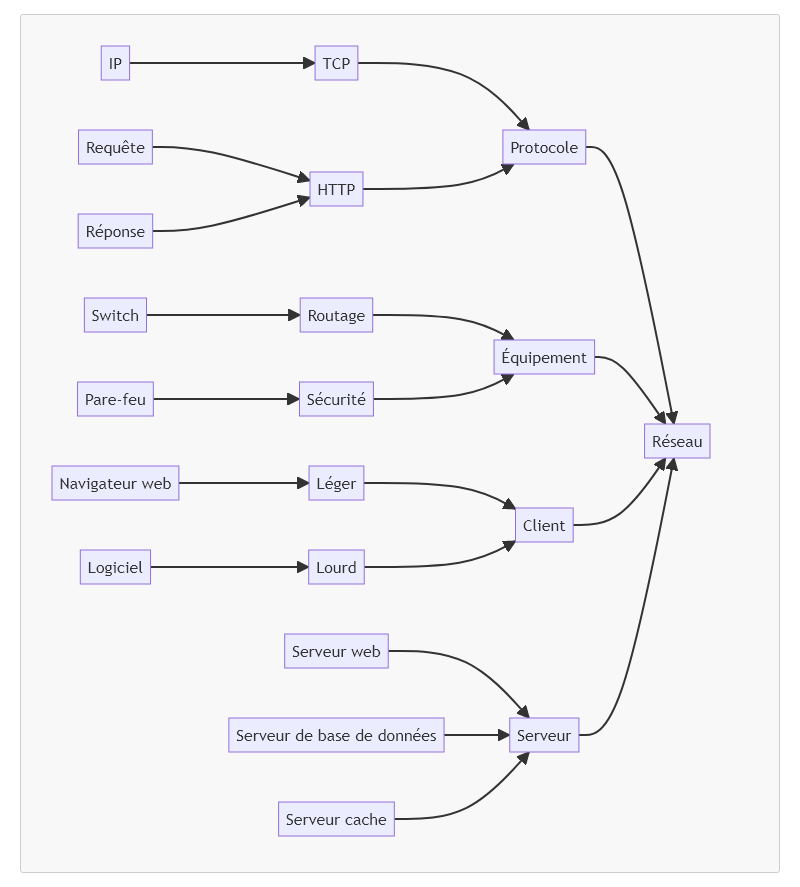
\includegraphics[width=\textwidth, height=\dimexpr\textheight-6.3cm\relax, keepaspectratio]{../images/mermaid_v1.png}
    \caption{Taxonomie simplifiée d'une relation client-serveur}
    \label{fig:Schéma de la taxonomie}
\end{figure}

\section{Ajout d'instances}

\subsection{Réseau}
\begin{itemize}
    \item IP : IPv4, IPv6
    \item Requête : GET, POST
    \item Réponse : 200, 404
\end{itemize}

\subsection{Client}
\begin{itemize}
    \item Navigateur : Chrome, Firefox
\end{itemize}

\subsection{Serveur}
\begin{itemize}
    \item Serveur Web : Nginx, IIS
    \item Serveur de base de données : MySQL, SQLServer
    \item Serveur cache : Redis, Memcached
\end{itemize}

\section{Ajout de prédicats}
\begin{figure}[ht]
    \centering
    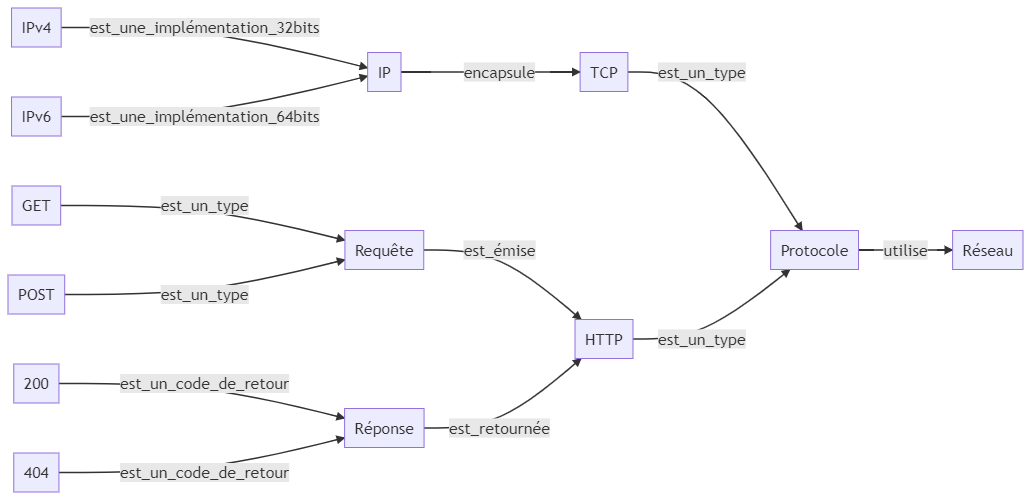
\includegraphics[width=\textwidth, height=\textheight, keepaspectratio]{../images/mermaid_v2_sub.png}
    \caption{Sous-graphe de la taxonomie simplifiée}
    \label{fig:Sous-graphe référençant les prédicats}
\end{figure}

\newpage
\section{Changements additionnels}
La représentation graphique de la taxonomie comporte des prédicats entre tous les noeuds.
\begin{figure}[ht]
    \centering
    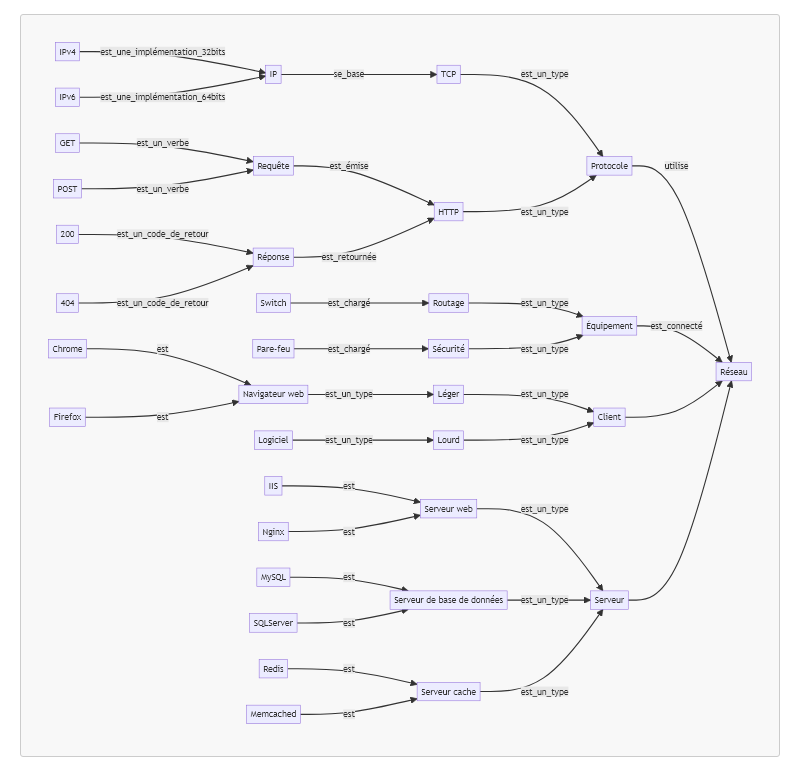
\includegraphics[width=\textwidth, height=\textheight, keepaspectratio]{../images/mermaid_v3.png}
    \caption{Graphe de la taxonomie mis à jour}
    \label{fig:Graphe de la taxonomie avec tous les prédicats}
\end{figure}

\end{document}